\documentclass[onecolumn,authoryear]{els-mrw}

\usepackage{amsmath,amssymb,amsfonts,amsthm,makeidx,graphicx}
\usepackage{txfonts}
\usepackage{helvet}

%%Please add any additional required packages before this commented line.

\begin{document}

\chapter{Main-sequence systems: tidal evolution}\label{chap1}

\author[1]{Kaloyan Penev}%

\address[1]{\orgname{The University of Texas at Dallas}, \orgdiv{Department of
Physics}, \orgaddress{Richardson, TX}}

\articletag{
%
    Chapter Article tagline: update of previous edition,, reprint..
%
}

\maketitle


\begin{glossary}[Glossary]
\term{Europe} the model is a coherent view of capital markets data that allows users to interact with the content in a consistent manner.

\term{Primates} regardless of the source. Essentially, of sources. Properly deployed.

\end{glossary}

\begin{glossary}[Nomenclature]
\begin{tabular}{@{}lp{34pc}@{}}
AF &Assessment Factor\\
ECHA &European Chemical Agency\\
EPM &Equilibrium Partitioning Method Equilibrium Partitioning Method Equilibrium Partitioning Method Equilibrium\hfill\break Partitioning Method\\
ERA &Ecological Risk Assessment\\
HC &Hazardous Concentration\\
\end{tabular}
\end{glossary}

Although the typical acquirer underperforms the market in the long term, not all acquisitions
destroy value. We search for factors that could help investors screen for valueenhancing
acquirers. For instance, cash-financed deals within the same industry involve
relatively large targets, enjoying better fortunes, and bidders who trade short-term market
reaction to the deal announcement are also important leading indicators.

\begin{abstract}[Abstract]

The easiest exoplanets to detect are those that orbit very close to their host
stars. As a result, even though these planets are quite rare, they represent a
major fraction of the current exoplanet population. A side-effect of the
proximity between the planet and the star is that the two have strong mutual
interactions through a number of physical processes. One of the most important
of these processes is tides. Tides are thought to shape the orbits of close-in
exoplanets, heat the planet making its radius expand, and even drive some
planets to spiral into their host stars. This chapter briefly introduces the
basics of tidal physics and describes the various fingerprints tides leave
within the observed exoplanet population.

\end{abstract}


\section{Introduction}
%
\label{sec:introduction}

The term tides refers to changes in the shape of an astronomical object (in our
case a planet or a star) in response to differences in the gravitational pull of
a nearby mass at different locations within the object. Below, tides and their
effects are discussed qualitatively. For a full mathematical description of
tides see \cite{Murray_Dermott_book}.

Consider an exoplanet system consisting of a single planet orbiting a single
star in a circular orbit. The gravitational acceleration due to the star at the
location of the planet's center provides the centripetal acceleration needed to
keep the planet in orbit. The part of the planet facing the star is closer to
the star and therefore experiences a slightly stronger gravitational pull.
However, if we ignore the rotation of the planet for a moment, that part of the
planet must follow a path with the same radius and period as the center of the
planet (though with its center offset slightly). The result is that the star
provides larger gravitational acceleration to that part of the planet than the
required centrifugal acceleration. This excess force as referred to as the tidal
force, and it is directed towards the star for the star-facing part of the
planet. Similarly, on the far side of the planet, the star's gravity is slightly
smaller than what is required to keep that part of the planet in orbit,
resulting in a tidal force pointing away from the star. These tidal forces cause
the planet to elongate along the star-planet line, and squeeze in the
perpendicular direction. This elongation is frequently referred to as the tidal
bulge.

Let us now consider the rotation of the planet. If the period of rotation is
exactly equal to the orbital period (a.k.a. synchronous rotation), the
sub-stellar point is fixed on the planet's surface, and consequently the tidal
bulge is also fixed relative to the planet. However, if the rotation and orbital
periods differ, the tidal bulge will travel on the planet's surface. If the
rotational angular velocity of the planet is $\Omega_{pl}$, and the orbital
angular velocity is $\Omega_{orb}$, a point on the surface of the planet will
travel at a rate of $\Omega_{orb} - \Omega_{pl}$ relative to the sub-stellar
point. Since there are two tidal bulges on the planet (one on the side facing
the star and one on the opposite side), the planetary material will experience a
tidal wave with a frequency of $2(\Omega_{orb} - \Omega_{pl})$.

Any time dependent deformation of the planet will be subject to some amount of
energy dissipation. The exact physical processes leading to this dissipation and
the amount of energy dissipation they drive depend on the internal structure and
properties of the planet. Regardless of the causes, this energy dissipation
introduces a delay between the tidal forcing and the response of the planet to
that forcing. If the planet spins faster than synchronous (i.e. $\Omega_{pl} >
\Omega_{orb}$), the tidal bulge will be ahead of the sub-stellar point, and if
$\Omega_{pl} < \Omega_{orb}$, the tidal bulge will lag behind
(Fig.~\ref{fig:tidal_bulge}).

\begin{figure}[t]
%
    \centering
%
    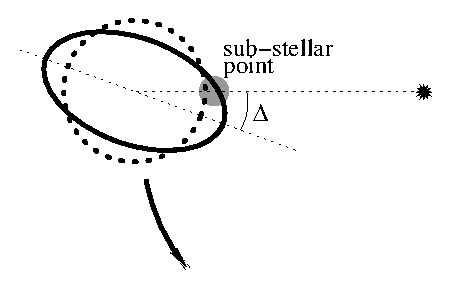
\includegraphics[width=0.5\textwidth]{tidal_bulge.eps}
%
    \caption{
%
        Exaggerated tidal bulge on a planet orbiting a star. Assuming that the
        planet spin angular velocity is smaller than than the orbital angular
        velocity, the tidal bulge will lag behind the sub-stellar point by an
        angle $\Delta$.
%
    }
%
    \label{fig:tidal_bulge}
%
\end{figure}

The two tidal bulges, now shifted relative to the star-planet line, will
experience the gravitational pull of the star. Since the closer bulge will feel
a stronger gravitational force than the farther bulge, there will be a net
torque on the planet. If the bulge is carried ahead of the sub-stellar point by
rotation, the gravitational pull of the star will apply a torque to the planet
opposite to its rotation, acting to slow down its spin, and the reaction force
on the star will act to add angular momentum to the orbit. Conversely, if the
tidal bulge lags behind the sub-stellar point, the gravitational pull of the
star will act to spin the planet up, taking angular momentum out of the orbit.

The discussion above assumed that the equator of the planet is aligned with the
orbital plane. This is not necessarily the case. If the planet's spin is tilted
with respect to the orbit, regardless of whether the planet is rotating faster
or slower than the orbit, rotation will shift the bulges away from the
sub-stellar point. This in turn will result in a torque that will tend over time
to bring the planet's equator and the orbital plane into alignment.

So far we only considered circular orbits. For non-circular orbits, the orbital
angular velocity is no longer constant. It is highest near periapsis (closest
approach between the planet and star) and lowest near apoapsis (largest
planet-star distance). In this case, tides will push the spin of the planet to a
state where the average torque over an orbit vanishes. This is known as
pseudo-synchronous rotation. Near periapsis the orbital angular velocity is
smaller than the pseudo-synchronous spin of the planet, thus the tidal bulge
leads the sub-stellar point, causing angular momentum to flow from the planet to
the orbit. Then for the part of the orbit around periapsis, the orbital angular
velocity exceed the pseudo-synchronous spin of the planet, causing angular
momentum to flow in the opposite direction. Since tides are stronger near
periapsis, the pseudo-synchronous period is somewhat shorter than the orbital
period, resulting in the planet being spun-down over a larger fraction of the
orbit, but at a slower rate.

For eccentric orbits, even if the planet is pseudo-synchronized, tidal
dissipation does not vanish, because the planet-star distance varies over time,
and the sub-stellar point is not fixed on the surface. From the discussion about
pseudo-synchronous period above, it is evident that near periapsis, the
sub-stellar point will drift eastward, and near apoapsis it will drift westward,
with a long-term westward average, since the pseudo-synchronous spin period is
shorter than the orbital period. These shifting both in location and amplitude
tidal bulges will still experience friction. Thus while no angular momentum will
be exchanged between the planet and the orbit, energy will be extracted from
the system and dissipated as heat, causing the orbit to circularize over time.

Everything we have said so far about the tides the star raises on the planet
applies equally to the tides the planet raises on the star. For circular orbits,
aligned with the stellar equator, if the spin angular velocity of the star
exceeds the orbital angular velocity, angular momentum is transferred from the
stellar spin to the orbit, and if the stellar spin is slower than the orbit,
angular momentum flows in the opposite direction. Similarly, we can define a
pseudo-synchronous period for the star at which the net tidal torque averaged
over a complete orbit vanishes. Even if the star is spinning
pseudo-synchronously, tidal energy dissipation continues and acts to circularize
the orbit over time. For misaligned orbits, tides will gradually work to align
the orbital plane with the stellar equatior.

The amplitude of the tidal bulge is set by competition between the tidal force
and the self-gravity of the planet or the star experiencing the tides.
Consequently, the planetary tides are positively correlated with the planet
radius and stellar mass and negatively correlated with the planet mass.
Conversely, the stellar tides are larger the larger the mass of the planet.
Finally, both stellar and planetary tides get weaker with increasing
star-planet separation, implying that tides will only be important if the planet
gets close to its parent star for at least some part of its orbit. This can
occur in one of two ways: either the planet has a very small orbital semimajor
axis (short period orbit), or the eccentricity of the planet is very large
making the pericenter distance small.

\section{Tidal Timescales}

Based on the discussion above, we can think of four separate tidal evolution
timescales:

\begin{enumerate}
%
    \item The timescale on which the planet's spin gets pseudo-synchronized and
        aligned with the orbit
%
    \item The timescale on which the orbit circularizes
%
    \item The timescale on which the orbital period of a circular orbit changes
%
    \item The timescale on which the stellar spin changes
%
\end{enumerate}

In order to compare some of these timescales, we need to consider the relative
angular momenta of the planet's spin, the orbit, and the stellar spin.

The planet's spin angular momuntum is negligible compared to both the orbital
angular momentum and the spin angular momentum of the star.  Consequently, both
the direction and period of the planet's spin can be changed by tides without
significantly affecting the orbit, implying that the timescale on which the
planet's spin gets pseudo-synchronized and aligned with the orbit is negligible
compared to the timescales on which the orbit or the stellar spin evolve. Thus,
we can assume that if a given exoplanet orbits close enough to its star for
tides to be important, to a good approximation we can assume that the planet's
spin is aligned with the orbit and pseudo-synchronized.

To compare the two timescales on which the orbit changes, we begin by comparing
the importance of the planetary to the stellar tides. The tidal deformation of
an object is set by a competition between the tidal force due to the companion
and the self-gravity of the object being tidally stretched. Since the planet has
a smaller self-gravity and experiences much larger tidal force than the star,
the planet is much more tidally deformed than the star. Consequently, as long as
planetary tides are not static they will drive faster orbital evolution than the
stellar tides. By the reasoning above, for both circular and eccentric orbits,
we expect the planet to be aligned and spin pseudo-synchronously with the orbit.
Hence, for eccentric orbits, the planetary tides still contribute to the
evolution, while for circular orbits they do not. This in turn means that the
tidal circularization timescale is shorter than the timescale on which circular
orbits change their period, since the latter is only driven by the much weaker
stellar tides.

To compare these timescales to the timescale on which the stellar spin is
affected by tides, note that stars have sufficiently large moment of inertia
for their spin angular momentum to be comparable to or larger than the orbital
angular momentum. Since only the stellar tides can affect the stellar spin, this
implies that the timescale on which the stellar spin changes is comparable to or
longer than the timescale on which the orbital period changes.


\section{Level 1 heading in sentance case}\label{chap1:sec1}

The results of this research are largely equivocal since body image is such a personal
concept, however some research suggests that appearance-related issues may, to some
extent, be influenced by treatment, age-related ordemographic details. For example,
younger patients with head and neck cancer have reported higher levels of anxiety
prior to disfiguring surgery\footnote{Gases and aerosols that move into or out of the
Earth's land and water bodies and those that are lost to space are
presumed to have an inconsequential effect on the mass present.} and more concerns around body image and sexuality have
beenreported by younger patients with breast, colon, testicular, female reproductive or
lymphatic cancer than by older patients with the same disease.

Where is the internuclear distance between spins, are the gyromagnetic
The angular portyion of the dipolar Hamiltonian is described using the second rank
Legendre function which is a function of the angle uij subtended by the magnetic field.
The psychosocial impact of an altered appearance after cancer can be far-reaching and
varied. As to the (negative) relationship between profits and share prices with respect to M\&As, see profits and
share prices with respect \cite{bib1}.

Where is the internuclear distance between spins, are the gyromagnetic
The angular portyion of the dipolar Hamiltonian is described using the second rank
Legendre function which is a function of the angle uij subtended by the magnetic field.
The psychosocial impact of an altered appearance after cancer can be far-reaching and
varied. Not only do patients have to contend with a new body image, \cite{bib2} they must also
deal with their feelings towards the loss of their previous looks.

\subsection{Level 2 heading in sentance case}\label{chap1:subsec1}

The results of this research are largely equivocal since body image is such a personal
concept, however some research suggests that appearance-related issues may, to some
extent, be influenced by treatment, age-related ordemographic details. For example,
younger patients with head and neck cancer have reported higher levels of anxiety
prior to disfiguring surgery and more concerns around body image and sexuality have
beenreported by younger patients with breast, colon, testicular, female reproductive or
lymphatic cancer than by older patients with the same disease.

\subsubsection{Level 3 heading in sentance case}\label{chap1:subsubsec1}

The results of this research are largely equivocal since body image is such a personal
concept, however some research suggests that appearance-related issues may, to some
extent, be influenced by treatment, age-related ordemographic details. For example,
younger patients with head and neck cancer have reported higher levels of anxiety
prior to disfiguring surgery and more concerns around body image \cite{bib3} and sexuality have
beenreported by younger patients with breast, colon, testicular, female reproductive or
lymphatic cancer than by older patients with the same disease.

\paragraph{Level 4 heading in sentance case}

The results of this research are largely equivocal since body image is such a personal
concept, however some research suggests that appearance-related issues may, to some
extent, be influenced by treatment, age-related ordemographic details. For example,
younger patients with head and neck cancer have reported higher levels of anxiety
prior to disfiguring surgery and more concerns around body image and sexuality have
beenreported by younger patients with breast, colon, testicular, female reproductive or
lymphatic cancer than by older patients with the same disease. To be in equilibrium, the intensity
of radiation cannot be dependent on direction (i.e., radiation must be
\emph{isotropic}), and temperature cannot depend on the frequency and
direction of electromagnetic radiation \cite{bib4}.

\subparagraph{Level 5 heading in sentance case}%

The results of this research are largely equivocal since body image is such a personal
concept, however some research suggests that appearance-related issues may, to some
extent, be influenced by treatment, age-related ordemographic details. For example,
younger patients with head and neck cancer have reported higher levels of anxiety
prior to disfiguring surgery and more concerns around body image and sexuality have
beenreported by younger patients with breast, colon, testicular, female reproductive or
lymphatic cancer than by older patients with the same disease.

\subsubparagraph{Level 6 heading in sentance case}%

The results of this research are largely equivocal since body image is such a personal
concept, however some research suggests that appearance-related issues may, to some
extent, be influenced by treatment, age-related ordemographic details.

\subsubsubparagraph{Level 7 heading in sentance case}%

The results of this research are largely equivocal since body image is such a personal
concept, however some research suggests that appearance-related issues may, to some
extent, be influenced by treatment, age-related ordemographic details.

\section{Display Math}\label{chap1:sec4}

All factors were found to be statistically significant. The goodness of fit from the
regression is also quite satisfactory. The six factors we used are capable of explaining
about 6\% of the return variability. The intercept from the regression is negative,
confirming that the average acquirer under performs the market. The long-term returns
of acquirers, however, are positively associated with the short-term market reaction,
the relative size of the target, and the valuation attractive be an indication
of a value enhancing
or a value-destroying acquisition.
\begin{align}\label{chap1:eq1}
p[m_1]+\cdots+p[m_2]=p[n_1]+\cdots+p[n_2]
\end{align}

In this chapter, we provide an overview of the theory of population games and deterministic evolutionary dynamics.  We introduce population games through a series of examples and illustrate their basic geometric properties.  We formally derive deterministic evolutionary dynamics from revision protocols, introduce the main families of dynamics---imitative/biological, best response, comparison to average payoffs, and pairwise comparison and discuss their basic properties.
\begin{align}\label{chap1:eq2}
\mathrm{{H_{2}}^{+}} + \mathrm{e}^{-} & \rightarrow  \mathrm{H} + \mathrm{H}, \\
\mathrm{HeH^{+}} + \mathrm{e}^{-} & \rightarrow  \mathrm{He} + \mathrm{H}.\label{chap1:eq3}
\end{align}

In this chapter, we provide an overview of the theory of population games and deterministic evolutionary dynamics.  We introduce population games through a series of examples and illustrate their basic geometric properties.  We formally derive deterministic evolutionary dynamics from revision protocols, introduce the main families of dynamics---imitative/biological, best response, comparison to average payoffs, and pairwise comparison and discuss their basic properties.

\begin{figure}[t]
\centering

\includegraphics[width=.4\textwidth]{blankfig}
\caption{A conservation relationship can also be written for electric charge, but in mesoscale modeling, electromagnetic effects are not considered to be dynamically or thermodynamically important on the model-resolved mesoscale. They are certainly important on  cloud and precipitation microphysics, and can therefore affect mesoscale
and larger processes, but this would need to be included through.}
\label{chap1:fig1}
\end{figure}

\section{Lists}\label{chap1:sec5}%
Deterministic evolutionary dynamics (See the \eqweblink{Equations}{chap1:eq1} and \eqref{chap1:eq2})  reflect the character of the protocols that generate them; for example, dynamics based on imitation are readily distinguished from those based on optimization \cite{bib5}.

These principles form a coupled set of relations that must be
satisfied simultaneously and that include sources and sinks in the
individual expressions.
\begin{itemize}%
\item The atmosphere is dry with no phase changes of water occurring.
\item Comparatively short time periods are involved so that radiational
heating or cooling of the air is relatively small.
\begin{itemize}%
\item conservation of motion,
\item conservation of water, and
\begin{itemize}%
\item conservation of mass,
\item conservation of heat,
\end{itemize}
\item conservation of other gaseous and aerosol materials.
\end{itemize}
\item The heating or cooling of the lowest levels of the atmosphere by
the bottom surface is of comparatively small magnitude.
\end{itemize}%%
Nevertheless, in some classes of games, dynamics derived from a variety of choice principles exhibit qualitatively similar behavior.
\begin{enumerate}%
\item The atmosphere is dry with no phase changes of water occurring.
\item Comparatively short time periods are involved so that radiational
heating or cooling of the air is relatively small.
\begin{enumerate}[a.]%
\item conservation of motion,
\item conservation of water, and
\begin{enumerate}%
\item conservation of motion,
\item conservation of other gaseous and aerosol materials.
\end{enumerate}
\item conservation of other gaseous and aerosol materials.
\end{enumerate}
\item The heating or cooling of the lowest levels of the atmosphere by
the bottom surface is of comparatively small magnitude.
\end{enumerate}%%

The expression for work in \eqweblink{Eq.}{chap1:eq3} could also have included external
work performed by such processes as \nobreak chemical reactions, phase changes,
or electromagnetism; however, these effects are not included in this
derivation of work.
\begin{unenumerate}%%
\item The atmosphere is dry with no phase changes of water occurring.
\item Comparatively short time periods are involved so that radiational
heating or cooling of the air is relatively small.
    \begin{unenumerate}%%
    \item conservation of motion. The heating or cooling of the lowest levels of the atmosphere\index{atmosphere} by
    the bottom surface is of comparatively small magnitude.
    \begin{unenumerate}%%
    \item conservation of water, and the heating or cooling of the lowest levels of the atmosphere by
    the bottom surface is of comparatively small magnitude.
    \item conservation of other gaseous and aerosol materials. The heating or cooling of the lowest levels of the atmosphere by
    the bottom surface is of comparatively small magnitude.
    \end{unenumerate}%%
\item The heating or cooling of the lowest levels of the atmosphere by
the bottom surface is of comparatively small magnitude.
    \end{unenumerate}
\item The heating or cooling of the lowest levels of the atmosphere by
the bottom surface is of comparatively small magnitude.
\end{unenumerate}%%
The ideal gas law, referred to previously, was derived from
observations of the behavior of gases at different pressures,
temperatures, and volumes \cite{bib6}.
\begin{description}
\item[A setup-time $T_c$ per pair of nuclear centers.] For interelectron repulsion
  integrals, the matrix $J_{\mu'\mu}({\mathbf{S}})$ evaluated as well.  For a
  molecule with $M$ atoms, this is done at most $M(M+1)/2$ times but
  fewer if nuclear displacements are repeated, or if symmetry
  reductions can be exploited.
\item[A setup time $T_2$ for each orbital density]  For each orbital density, the expansion
  coefficients $c_{\tau_1,\tau_2}^\tau$ are initialized. For
  one-particle integrals, nothing else needs to be done for this
  step. For the interelectron repulsion integrals.
\item[Computation time per interelectron repulsion integral $T_4$] For every integral, the final dot product is performed.
\end{description}
Investigators in the 17th and 18th
centuries found that, for a given gas, pressure times volume equals a
constant at any fixed temperature (Boyle's law) and that pressure
divided by temperature equals a constant at any fixed volume
(Charles's law). These two relations can be stated more precisely as
\begin{quote}
\quotehead{Quotehead}
The foundation for any model is a set of conservation principles. For mesoscale atmospheric models, these principles are conservation of mass, conservation of heat, conservation of motion, conservation of water, the conservation of other gaseous and aerosol materials, and an equation of state.
\source{--source}
\end{quote}
The ideal gas law, referred to previously, was derived from
observations of the behavior of gases at different pressures,
temperatures, and volumes. Investigators in the 17th and 18th
centuries found that, for a given gas, pressure times volume equals a
constant at any fixed temperature (Boyle's law) and that pressure
divided by temperature equals a constant at any fixed volume
(Charles's law). These two relations can be stated more precisely as

\begin{figure}[b]
\centering

\includegraphics[width=0.65\textwidth]{blankfig}
\caption{A conservation relationship can also be written for electric charge, but in mesoscale modeling, electromagnetic effects are not considered to be dynamically or thermodynamically important on the model-resolved mesoscale.}
\label{chap1:fig2}
\end{figure}

\section{Floats}\label{chap1:sec6}
The value of the gas constant $R$ for different gases is determined
using Avogadro's hypothesis that at a given temperature and pressure
gases containing the same number of molecules occupy the same
volume. From experimental work, for example, it has been shown that at
a pressure of 1 atm ($P_0 = 1014$ mb) and a temperature of $T_0 = 273$
K, 22.4 kliter of a gas ($V_0$) will have a mass in kilograms equal to
the molecular weight of the gas $\mu$. This quantity of gas is defined
as 1 kmol. A conservation relationship can also be written for electric charge, but in mesoscale modeling, electromagnetic effects are not considered to be dynamically or thermodynamically important on the model-resolved mesoscale. They are certainly important on  cloud and precipitation microphysics, and can therefore affect mesoscale and larger processes, but this would need to be included through~parameterizations of the microphysics.
In this chapter, we provide an overview of the theory of population games and deterministic evolutionary dynamics.  We introduce population games through a series of examples and illustrate their basic geometric properties.  We formally derive deterministic evolutionary dynamics from revision protocols, introduce the main families of dynamics---imitative/biological, best response, comparison to average payoffs, and pairwise comparison and discuss their basic properties \cite{bib7}.

In this chapter, we provide an overview of the theory of population games and deterministic evolutionary dynamics.  We introduce population games through a series of examples and illustrate their basic geometric properties.  We formally derive deterministic evolutionary dynamics from revision protocols, introduce the main families of dynamics---imitative/biological, best response, comparison to average payoffs, and pairwise comparison and discuss their basic properties.
In this chapter, we provide an overview of the theory of population games and deterministic evolutionary dynamics.  We introduce population games through a series of examples and illustrate their basic geometric properties.  We formally derive deterministic evolutionary dynamics from revision protocols, introduce the main families of dynamics---imitative/biological, best response, comparison to average payoffs, and pairwise comparison and discuss their basic properties.
\begin{table}[t]
\TBL{\caption{Molecular weight and fractional contribution by mass
of major gaseous components of the atmosphere}\label{chap1:tab1}}
{\begin{tabular*}{\textwidth}{@{\extracolsep{\fill}}@{}lll@{}}
\toprule
\multicolumn{1}{@{}l}{\TCH{Gas}} &
\multicolumn{1}{c}{\TCH{Molecular weight\footnotemark{a}}} &
\multicolumn{1}{l}{\TCH{Fractional contribution by mass}}\\
\colrule
N$_2$ & 28.016 & 0.7551\\
O$_2$ & 32.00\phantom{6} & 0.2314\\
Ar & 39.94\phantom{6} & 0.0128\\
H$_2$O & 18.02\phantom{6} & variable\\
\botrule
\end{tabular*}}{%
\begin{tablenotes}
\footnotetext[a]{Table footnote text...}
\footnotetext{\source{Table source text...}}
\end{tablenotes}
}%
\end{table}
In this chapter, we provide an overview of the theory of population games and deterministic evolutionary dynamics.  We introduce population games through a series of examples and illustrate their basic geometric properties.  We formally derive deterministic evolutionary dynamics from revision protocols, introduce the main families of dynamics---imitative/biological, best response, comparison to average payoffs, and pairwise comparison and discuss their basic properties.
In this chapter, we provide an overview of the theory of population games and deterministic evolutionary dynamics.  We introduce population games through a series of examples and illustrate their basic geometric properties.  We formally derive deterministic evolutionary dynamics from revision protocols, introduce the main families of dynamics---imitative/biological, best response, comparison to average payoffs, and pairwise comparison and discuss their basic properties.

\begin{table}%% Coding for Non-floating table
\TBL{\caption{Table caption}}{%
\begin{tabular*}{\columnwidth}{@{\extracolsep\fill}ll@{}}
\toprule
\multicolumn{1}{@{}l}{\TCH{Gas}} &
\multicolumn{1}{c}{\TCH{Molecular weight}} \\
\colrule
N$_2$ & 28.01 \\
O$_2$ & 32.00\\
Ar & 39.94\\
H$_2$O & 18.02\\
\botrule
\end{tabular*}}{}
\end{table}

In this chapter, we provide an overview of the theory of population games and deterministic evolutionary dynamics.  We introduce population games through a series of examples and illustrate their basic geometric properties.  We formally derive deterministic evolutionary dynamics from revision protocols, introduce the main families of dynamics---imitative/biological, best response, comparison to average payoffs, and pairwise comparison and discuss their basic properties.

\section{Boxed Text}\label{chap1:sec7}%

When water vapor is included, the apparent molecular weight can be
written as where $q$ is the specific humidity or ratio of the mass of water vapor
$M$, to the mass of dry air $M_{\mathrm{d}}$. Expanding this relation This form of the ideal gas law includes the contribution of water
vapor and is often written as

Stated another way, this concept requires that the
mass into and out of an infinitesimal box must be equal to the change
of mass in the box. Such a volume is sketched,
where $\rho u|_1 \, \delta y \, \delta z$ is the mass flux into the left side
and $\rho u|_2 \,
 \delta y \, \delta z$ the mass flux out of the right side. The
symbols $\delta x$, $\delta y$, and $\delta z$ represent the
perpendicular sides of the box,  $\rho$ the density, and $u$ the velocity
component normal to the $\delta z \, \delta y$ plane.
In the Earth's atmosphere, mass is assumed (See \weblink{Boxes}{chap1:box1} and Text \weblink{Box}{chap1:box1}) to have neither sinks nor the
sources.

\begin{BoxTypeA}[chap1:box1]{Box head}
\section*{Box 1 hd}
Stated another way, this concept requires that the
mass into and out of an infinitesimal box must be equal to the change
of mass in the box. Such a volume is sketched,
where $\rho u|_1 \, \delta y \, \delta z$ is the mass flux into the left side
and $\rho u|_2 \,
 \delta y \, \delta z$ the mass flux out of the right side.

\subsection*{Box 2 hd}
The
symbols $\delta x$, $\delta y$, and $\delta z$ represent the
perpendicular sides of the box,  $\rho$ the density, and $u$ the velocity
component normal to the $\delta z \, \delta y$ plane.
In the Earth's atmosphere, mass is assumed to have neither sinks nor the
sources.

Stated another way, this concept requires that the
mass into and out of an infinitesimal box must be equal to the change
of mass in the box.

Such a volume is sketched,
where $\rho u|_1 \, \delta y \, \delta z$ is the mass flux into the left side
and $\rho u|_2 \,
 \delta y \, \delta z$ the mass flux out of the right side. The
symbols $\delta x$, $\delta y$, and $\delta z$ represent the
perpendicular sides of the box,  $\rho$ the density, and $u$ the velocity
component normal to the $\delta z \, \delta y$ plane.
In the Earth's atmosphere, mass is assumed to have neither sinks nor the
sources.

Stated another way, this concept requires that the
mass into and out of an infinitesimal box must be equal to the change
of mass in the box. Such a volume is sketched,
where $\rho u|_1 \, \delta y \, \delta z$ is the mass flux into the left side
and $\rho u|_2 \,
 \delta y \, \delta z$ the mass flux out of the right side.

 The
symbols $\delta x$, $\delta y$, and $\delta z$ represent the
perpendicular sides of the box,  $\rho$ the density, and $u$ the velocity
component normal to the $\delta z \, \delta y$ plane.
In the Earth's atmosphere, mass is assumed to have neither sinks nor the
sources.
\end{BoxTypeA}

The foundation for any model is a set of conservation principles. For mesoscale atmospheric models, these principles are conservation of mass, conservation of heat, conservation of motion, conservation of water, the conservation of other gaseous and aerosol materials, and an equation of state.

The foundation for any model is a set of conservation principles. For mesoscale atmospheric models, these principles are conservation of mass, conservation of heat, conservation of motion, conservation of water, the conservation of other gaseous and aerosol materials, and an equation of state.

\section{Enunciations}
\label{chap1:App1}
where $q_1, q_2$ and $q_3$ are defined as the ratio of the mass of the
solid, \cite{bib8} and \cite{bib9} liquid, and vapor forms of water, respectively, to the mass of
air in the same volume.
\begin{theorem}
The source-sink term $S_{q_{n}}$ refers to the
processes $\sum_{i=1}^{N} m_i\,{=}\, 1$. \eqweblink{Equation}{chap1:eq1} whereby water undergoes phase changes as well as to water
generated or lost in chemical reactions.
\end{theorem}
\begin{theorem}[Proof of Theorem]
The source-sink term $S_{q_{n}}$ refers to the
processes $\sum_{i=1}^{N} m_i\,{=}\, 1$. \eqweblink{Equation}{chap1:eq2} whereby water undergoes phase changes as well as to water
generated or lost in chemical reactions.
\end{theorem}
\begin{theorem*}
The source-sink term $S_{q_{n}}$ refers to the
processes $\sum_{i=1}^{N} m_i\,{=}\, 1$. \eqweblink{Equation}{chap1:eq3} whereby water undergoes phase changes as well as to water
generated or lost in chemical reactions.
\end{theorem*}
\begin{theorem*}[Proof of Theorem]
The source-sink term $S_{q_{n}}$ refers to the
processes $\sum_{i=1}^{N} m_i\,{=}\, 1$. \eqweblink{Equation}{chap1:eq3} whereby water undergoes phase changes as well as to water
generated or lost in chemical reactions.
\end{theorem*}
\begin{proof}
The source-sink term $S_{q_{n}}$ refers to the \cite{bib10}
processes whereby water undergoes phase changes as well as to water
generated or lost in chemical reactions.
\end{proof}
For most mesoscale
applications, chemical changes in water mass can be neglected and the
terms can be expressed as contributions owing to the following
processes:
\begin{definition}
The source-sink term $S_{q_{n}}$ refers to the
processes $\sum_{i=1}^{N} m_i\,{=}\, 1$. \eqweblink{Equation}{chap1:eq2} whereby water undergoes phase changes as well as to water
generated or lost in chemical reactions.
\end{definition}
For most mesoscale
applications, chemical changes in water mass can be neglected and the
terms can be expressed as contributions owing to the following
processes:
\begin{remark}
The source-sink term $S_{q_{n}}$ refers to the
processes $\sum_{i=1}^{N} m_i\,{=}\, 1$. \eqweblink{Equation}{chap1:eq1} whereby water undergoes phase changes as well as to water
generated or lost in chemical reactions.
\end{remark}

\begin{ack}[Acknowledgments]
The result of this approach is to produce a top-down view of tIt is a
framework that standardizes the manner in which organizations can
refer to complex data content, thereby reducing the overheads supports
an incremental approach to improving business applications and
operating efficiency. It can be applied as and when needed so the manner
in which organizations can refer to complex data content, thereby
reducing the overheads supports an incremental approach to improving
business applications and that new systems take on a standard.
\end{ack}

\seealso{article title article title}

\bibliographystyle{Harvard}
\bibliography{bibliography}

\end{document}

